\chapter{Generation} \label{chap:generation}
Synthetic data can have several forms. They can be textual, tabular or media-based. Artificial text-based data is very commonly used in sentence formation and automated voice-over (ex., amazon uses synthetic text data to bootstrap Alexa's language options \citep{kollar2018alexa}). An example of its usage can be seen in Fig. \ref{fig:genie}. Tabular data is the most common type of synthetic data. Its objective is to mimic real-life data stored in tables. An example of artificial tabular data is the one used by \cite{toutanova2016dataset} to create a synthetic dataset focused on language by hand. Lastly, we have synthetic media-based data. This data can be artificial video, image, or sound. Media is rendered with properties close-enough to real-life data. This similarity allows synthetic media to replace the original data as a drop-in replacement.

There are three types of artificially generated data. It is possible to subsample it from a synthetically generated population. This kind of generation is known as fully synthetic dataset generation. Theoretically, fully synthetic datasets provide 100\% guarantee against the disclosure of sensitive attribute value \citep{rubin1993statistical}.
Using an already existing dataset to generate a new dataset containing the original characteristics while artificially generating data used to replace sensitive values is also possible. This generation method is known as partially synthetic dataset generation. An imputer alters the values of a set of attributes for a subset of data points to protect sensitive information. This way, the actual values that contain a high risk of revelation are replaced \citep{dandekar2018comparative}. 
We can also generate data using both natural and synthetic data. To this kind, we give the name of hybrid synthetic data. We chose a close record in the synthetic data for each random record of actual data. Then both are combined to form hybrid data. It has the advantages of both fully and partially synthetic data. Therefore, it provides proper privacy preservation with high utility compared to the other two. Its generation requires extra steps, and as such, this type of synthetic data requires more memory and processing time.

The goal of dataset generation is to create a synthetic data generation method that is modular, repeatable, and automated. The synthetic data should be realistic enough that its measurements and performance are similar (and, as such predictive) to real-world data measurements and performance \citep{boggs2014synthetic}. One example of generator integration can be seen in Fig \ref{fig:genie}. This figure depicts an overview of the Genie Semantic Parser Generator, a toolkit for creating a semantic parser for new virtual assistant capabilities. In this generator sentences are synthetically created \citep{campagna2019genie}.



\begin{figure}
    \centering
    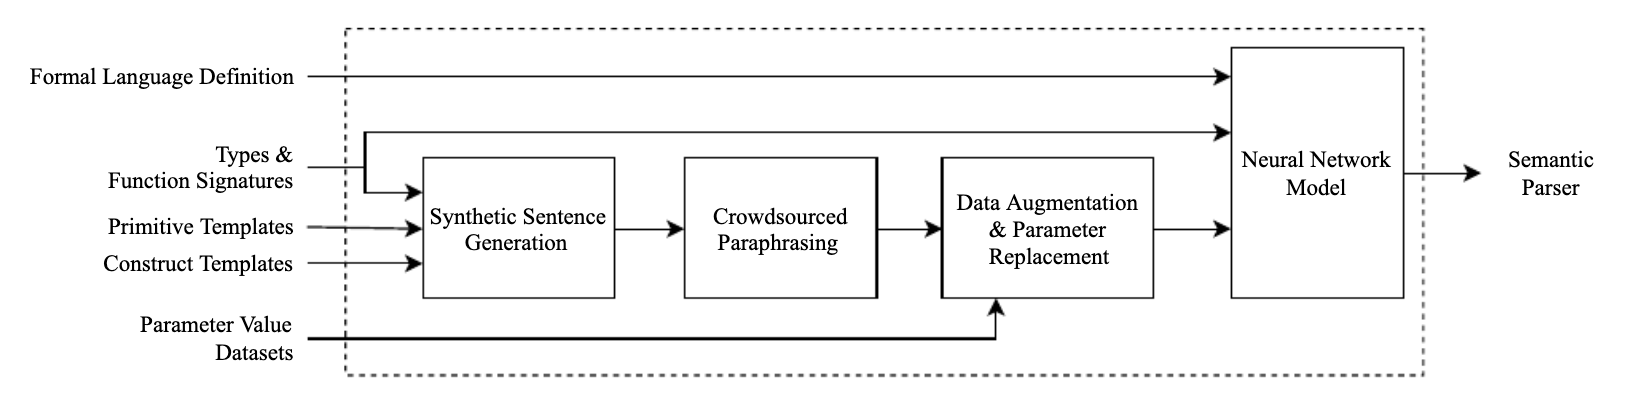
\includegraphics[width=\textwidth]{genie-vc.png}
    \caption[Overview of the Genie Semantic Parser Generator]{Overview of the Genie Semantic Parser Generator \citep{campagna2019genie}.}
    \label{fig:genie}
\end{figure}

A statistical distribution is the method typically used to generate synthetic data. This distribution is made for a set of samples from directly measured data. New values are created in the same format as the actual data. 

\cite{drechsler2010using} presented a procedure for synthetic dataset generation: "We define an order of the attributes that will be synthesised; values of the first attribute are synthesised by training the dataset synthesiser on the original dataset".

In the following sections, we will look at a series of dataset generation methodologies.

\section{Conditionial Distribution}
A conditional distribution is a distribution of values for one variable that exists when the values of other variables are specified. This distribution allows one to estimate the distribution of one's variable of interest under specific conditions.

The marginal probability (presented below) represents the probability of a single event occurring, independent of other events. On the other hand, a conditional probability represents the likelihood that an event occurs, given that another specific event has already occurred.

According to \cite{cond}, the aim of conditional distribution applied to dataset generation is that a random sample from the target conditional distribution can be obtained by the action of the conditional generator on a sample drawn from a reference distribution.

\section{Sampling from Independent marginals}
The Independent marginals method consists of sampling from the observed marginal distributions of each variable. Marginal probability is the name given to the probability of an event irrespective of the outcome of another variable \citep{indmargins}. 

The marginal distribution of a group of arbitrary variables is the probability distribution of the variables included in the group. It gives the likelihood of varied values of the variables in the group without reference to the values of the other variables. This distribution differs from a conditional distribution, which presents the probabilities considering the values of the other variables \citep{trumpler1953statistical}.

The independent marginals method approach has its advantages: it is computationally efficient. It possibly estimates marginal distributions for different variables in parallel. However, it does not capture statistical dependencies across variables. Therefore, the generated synthetic data may fail to capture the structure of the original data \citep{disclosure}.

\section{Bayesian network}
Bayesian networks are probabilistic graphical models. In these models, each node represents a random variable. The edges between the nodes represent probabilistic dependencies among the corresponding random variables. The graph structure and conditional probability distributions are inferred from the actual data \citep{baye}.

The learning process in Bayesian networks is comprised of two steps. The first one consists of learning a directed graph from the data. This graph expresses all the variables’ pairwise conditional dependencies (or lack thereof). The second step is estimating the conditional probability tables \citep{disclosure}.

The graph deduced from the actual data contains the conditional reliance among the variables. This graph also provides a visual representation of the variables’ relationships. By sampling from the inferred Bayesian network, we can generate synthetic data.

\section{Mixture of product of multinomials} %probably not gonna use this one
A multinomial experiment is a statistical experiment with a series of characteristics. The experiment consists of a set amount of repeatable trials. Each trial has a set number of outcomes and a constant probability for each outcome. These are independent, meaning that a previous trial does not influence future trials.

Any multivariate categorical data distribution can be expressed as a mixture of the product of multinomials (MPoM) \citep{dunson2009nonparametric}.

The multinomial model over term frequencies is defined in the Equation (\ref{eq:1}).

\begin{equation} \label{eq:1}
    P(\tilde{x}|\tilde{y}) =\frac{l!}{\prod _i x_{i}}\prod_{i=1}^{n}y_{i}^{x_{i}}
\end{equation}

where \(x_{i}\) is the number of times word \(i\) occurs, \(y_{i}\) is the mean parameter for word \(i\), and \(l=\sum _{i} x_{i}\) is the document length \citep{rennie2005mixtures}.

%We can view the multinomial as the following generative process. We have a hopper filled with balls. Each ball represents one of the n words and the hopper and balls are designed so that the chance of pulling a ball labeled word i is µi. Each hopper draw is a “word” event. Balls are replaced before the next draw. We tally word counts, but no not keep track of order information. The resulting set of counts is a “document” event.

Theoretical guarantees exist regarding the flexibility of this methodology to model any multivariate categorical data. However, this process can be very time-consuming in problems with large datasets.

%\section{Categorical latent Gaussian process}
%The categorical latent Gaussian process (CLGP) is a generative model for multivariate categorical data \cite{dunson2009nonparametric}. CLGP uses a lower dimensional continuous latent space and non-linear transformations for mapping the points in the latent space to probabilities (via softmax) for generating categorical values.

%Like BN and MPoM, CLGP is a fully generative Bayesian model, but has richer latent non-linear mappings that allows for representation of very complex full joint distributions. The inferred low-dimensional latent space in CLGP may be useful for data visualization and clustering.

%Inference for CLGP is considerably more complex than other models due to its non-conjugacy. An approximate Bayesian inference method such as variational Bayes (VB) is required.

%VB for CLGP requires several other approximations such as low-rank approximation for GPs as well as Monte Carlo integration. Hence, the inference for CLGP scales poorly with data size.

\section{Generative adversarial networks}
In the generative adversarial networks (GANs), two neural networks are trained jointly, competing. While the first network focuses on creating a realistic artificial dataset, the second tries to distinguish between natural and synthetic data from the first dataset. Due to the competition, each network pushes the other, leading to better results \citep{gans}. 

GANs have been successful in generating more complex data, being capable of producing synthetic images and text \citep{Mirza}. They are, however, incapable of producing categorical datasets. GANs cannot compute "gradients latent categorical variables for training vis backpropagation" - (in \cite{disclosure}). GANs do not require strict probabilistic models to perform their generation tasks. Therefore they are more flexible than the models previously mentioned. They can also deal with mixed data types.

When a GAN has many parameters, proper choice of multiple tuning ones (hyper-parameters) is difficult and time-consuming. GANs are also challenging to train. Solving the associated min-max optimization problem can be very unstable. This can, however, be circumvented if the variation Wasserstein GAN is applied \citep{gan}.

\begin{comment}
  
\section{Multiple imputation}
Multiple imputation is a method where several distinct possible datasets are created and the final dataset results from combining those datasets. This way, this approach is an optimal one to use in order to solve problems of missing data. 

The generation process starts with the creation of several copies of the dataset. These copies will have their missing values replaced by plausible imputed user values according to their original distribution.

The next set is the analysis of the created datasets. In this step, each dataset is analysed individually. This step is followed by combining these datasets in the proper output synthetical dataset.
\end{comment}

%The following sections are still transcribed and need to be rewritten and expanded
\section{Linear Regression}
Linear regression seeks to model the association between two variables by using a linear equation to the observed data. One variable is considered an explanatory variable, and the other is regarded as a dependent variable.

We can describe a linear regression line using the formula: \(Y = a + bX\). This formula's X is the explanatory variable, and Y is the dependent variable. The line slope is \textit{b}, and \textit{a} is the intercept (the value of \textit{y} when \textit{x = 0}).

To synthesise every attribute \(Y_{i}\) in a dataset, we learn the parameters of the regression model using the dataset with attributes in \(Y_{-i}\). We generate values for \(Y_{i}\) by sampling from a Gaussian distribution with constant variance and the mean as determined regression parameters.

\cite{regression} used linear regression to generate different datasets with the same estimates. This was developed for teaching purposes to demonstrate that different sets of regression data can give precisely the same estimated regression functions. 

\section{Decision Tree}
\cite{reiter2005using} proposed a generation technique that uses classification and regression tree. That author applied it to the generation of a partially synthetic dataset. The main components of a decision tree model are nodes and branches, and the most critical steps in building a model are splitting, stopping, and pruning \citep{song2015decision}.
\begin{figure}[t]
  \begin{center}
    \leavevmode
    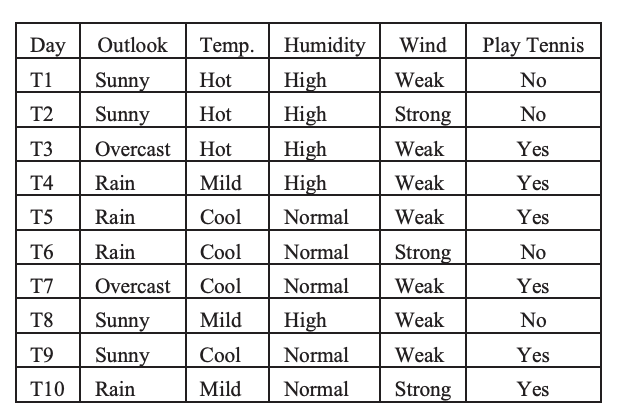
\includegraphics[width=0.5\textwidth]{dt_table.png}
    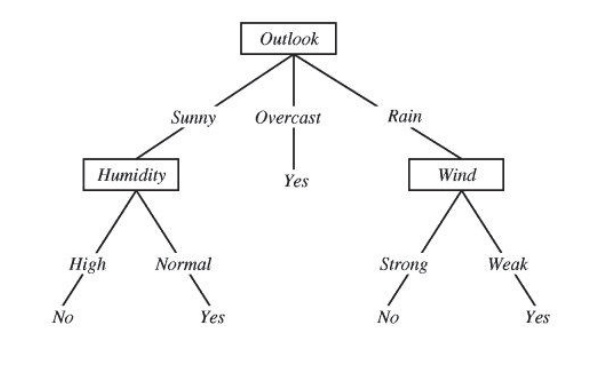
\includegraphics[width=0.5\textwidth]{dt_tree.png}
    \caption[Creation of a Decision Tree using a dataset]{Creation of a Decision Tree using a dataset [\cite{8226246}].}
    \label{fig:destree}
  \end{center}
\end{figure}

The process starts with building a decision tree using the values of the available attributes in the dataset \(Y-i\). To synthesise the value of an attribute \(Yi\) for a data point, we trace down the tree using the known attributes of the datapoint until reaching the leaf node. \cite{kirchner2004decision} applied this method to swine production and concluded that "the decision tree algorithm can detect relationships and patterns in real swine breeding datasets". Figure \ref{fig:destree} depicts a decision tree model created from a tabular dataset. An ML model was used to decide on a playing tennis binary problem. 


\section{Random Forecast}
Random Forest is a method introduced by \cite{breiman2001random}. As its name implies, a random forest consists of many individual decision trees that operate as a group. Each particular tree in the random forest releases a class prediction, and voting occurs for each class. The class with the most votes becomes our model’s prediction.

To synthesise values for a distinct point \(Yi\), a fixed number of decision trees on random samples of the training dataset \(Y-i\) are trained. The assemblage of results from the decision tree for a categorical attribute forms a multinomial distribution. For a continuous attribute, \cite{caiola2010random} propose using a kernel density estimator over the results from decision trees using sample values from the estimator.

\section{Neural Network}
Neural Networks are at the core of deep learning algorithms. They are inspired by the human brain, simulating how bodily neurons signal to one another \citep{abdi1999neural}.

Artificial neural networks (ANNs) incorporate node layers possessing an input layer, one or more hidden layers, and an output layer. Each node represents a neuron that connects to another and has an associated weight and target value (threshold). If the signal sent individual node is above the specified target value, that node is activated. Data is then sent to the next layer of the network.

Neural networks depend on training data to learn and improve accuracy over time. Nevertheless, once these learning algorithms are fine-tuned for precision, they are potent tools in computer science and artificial intelligence. This allows us to categorise and cluster data at a high rate.

%When looking at the dataset generation process, a neural network learns an abstract function mapping an input to the affiliated output as a data synthesiser. The output layer of a neural network incorporates K nodes (where K is the class classification problem). Each node represents the probability of the class being the model's output. We treat every attribute as a categorical variable. To synthesise the value of an attribute \(Yi\), we train a neural network using features in \(Yi-1\). We sample a value for attribute \(Yi\) using the output layer as a multinomial distribution.


\begin{comment}
  
\section{Evaluation}
One of the primary intents of enhancing a dataset generator is to increase the quality of the produced synthetic datasets. In order to evaluate the quality of a dataset, some methodologies are required.

The majority of evaluation functions use a scoring scheme. Let us suppose that D1 and D2 are datasets and \(E(x)\) is an evaluation function, and thus \(E(D1)\) and \(E(D2)\) generate some scores. If \(E(D1)>E(D2)\), we can expect that dataset D1 will yield better training/testing accuracy than D2.

\cite{dash1997feature} grouped evaluation functions into five categories: distance measures, information measures, dependency measures, consistency measures, and classifier error rate measures. Distance measures are the most popular and include separability, divergence, and discrimination measures. These measures were further analysed by \cite{4295518}. 

In the following sections, we will look at some evaluation approaches and points of interest when it comes to dataset evaluation.

\subsection{Distance Methods}
In this section, we summarize several distance measures for dataset evaluation. These measures are designed for feature evaluation, but they can be adopted for dataset evaluation. The goal of distance measurement is to calculate the distances among categories in a dataset.

\subsubsection{Euclidean distance}
The Euclidean distance between the two points \(p(p_{1}, p_{2}, p_{3}, …, p_{n})\) and \(q(q_{1}, q_{2}, q_{3}, …, q_{n})\) is defined as follows:

\begin{equation}
    d(p,q)=\sqrt{(p_{1}-q_{1})^2+(p_{2}-q_{2})^2+...+(p_{n}-q_{n})^2}
\end{equation}

Various equations can define Euclidean distance measure (EDM) for quantifying distance between two categories. One possible representation is:
\begin{equation}
    E(A,B)=d(c_{A},c_{B})-(r_{A}+r_{B})
\end{equation}

In this equation \(c_{A}\) and \(c_{B}\) are the center points of categories A and B. 
\(r_{A}\) and \(r_{B}\) are the radii of A and B. To calculate these values we can use the formula:
\begin{equation}
    r_{A}=\frac{1}{m}\sum_{i=1}^{m}d(c_{A},p_{i})
\end{equation}

Here \(m\) is the total number of points \(p_{i}\) and is a point in category A.

\subsubsection{Manhattan distance}
The Manhattan distance is similar to the Euclidian distance, but the distance between points \(p_{i}\) and \(q_{i}\) is calculated via a different equation.
\begin{equation}
    m(p,q)=\sum_{i=1}^{n}|p_{i}-q_{i}|
\end{equation}

Manhattan distance measure (MDM) can be defined as follows:
\begin{equation}
    M(A,B)=m(c_{A},c_{B})-(r_{A}+r_{B})
\end{equation}

\subsubsection{Hausdorff distance}
In mathematics, the Hausdorff distance, or Hausdorff metric, also called Pompeiu–Hausdorff distance \cite{birsan2005one}. It measures how far two subsets of a metric space are from each other. It turns the set of non-empty compact subsets of a metric space into a metric space in its own right. It is named after Felix Hausdorff and Dimitrie Pompeiu.

\begin{equation}
    \forall x_{1} \in A,D(x_{1},B) = min_{x_{2}\in B}\{d(x_{1},x_{2})\}
\end{equation}
\begin{equation}
    h(A,B) = max_{x_{1}\in A}\{D(x_{1},B)\}
\end{equation}
\begin{equation}
    H(A,B)=max\{h(A,B),h(B,A)\}
\end{equation}
These previous 3 equations display the needed steps for calculating the Hausdorff distance between set A and set B.

\(D(x_{1},B)\) is the distance between a point \(x_{1}\) in sets A and B, and \(d(x_{1},x_{2})\) means the distance between the two points \(x_{1}\) and \(x_{2}\). The directed function \(h(A, B)\) refers to the distance between set A and set B, and \(H(A, B)\) is also the distance between sets A and B. The Hausdorff Distance Measure (HDM) uses \(H(A, B)\) to calculate the distance among categories of a dataset.

\subsection{Comparison}
The measures presented before were analysed (alongside other metrics) by \cite{oh2011new}. They performed a series of analysis tests on 6 different datasets. The quality of this sets can be describe as follows: \(D_{1}>D_{2}>D_{3}>D_{4}>D_{5}>D_{6}\). The results can be seen in Fig. \ref{fig:dist_metrics}

\begin{figure}
  \begin{center}
    \leavevmode
    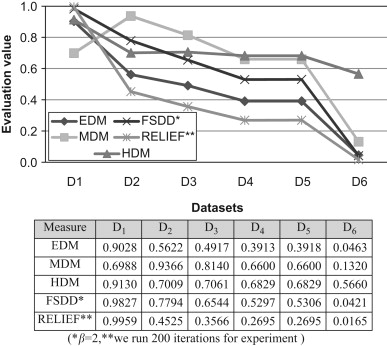
\includegraphics[width=0.7\textwidth]{metrics evaluation.jpg}
    \caption[Evaluation of distance metrics for dataset classification]{Evaluation of distance metrics for dataset classification \cite{oh2011new}}
    \label{fig:dist_metrics}
  \end{center}
\end{figure}
The relevant data to our study is the one related to the EDM (Euclidean distance measure), MDM (Manhattan distance measure) and HDM (Hausdorff Distance Measure). As we know that the datasets are numbered by highest quality to lowest quality, we can see that EDM proved more correct tham the others, with MDM having some problems with quantifying the quality of the 1st dataset and HDM performing the worst, being unable to identify major diferences betewenn the qualities if the datasets 2 to 5.

The other two methods displayed are used in feature selection.
\end{comment}

\section{Common dataset problems}
Other metrics exist that should be analysed when asserting the quality of a dataset. The usual suspects are overfitting, underfitting, missing data and data imbalances. In the following sections, we will look at these problems.

\subsection{Overfitting and Underfitting}
Overfitting might appear when a spurious pattern in the original dataset is captured and replicated with increasing frequency. This expands the amount of unnecessary random noise in the dataset. ML models trained with overfitted datasets are negatively impacted performance-wise. The random fluctuations of data are picked and learned as recurring moments \citep{over}.

Underfitting is the opposite of overfitting. It happens when the synthetic dataset does not capture enough relevant information from the original. Original metrics are not replicated, leading to a dataset with different distributions and metrics. ML models that used underfit datasets displayed poor performance ratios.

A graphical representation of overfitted and Underfitting can be found in Fig. \ref{fig:fitting}
\begin{figure}[!h]
  \begin{center}
    \leavevmode
    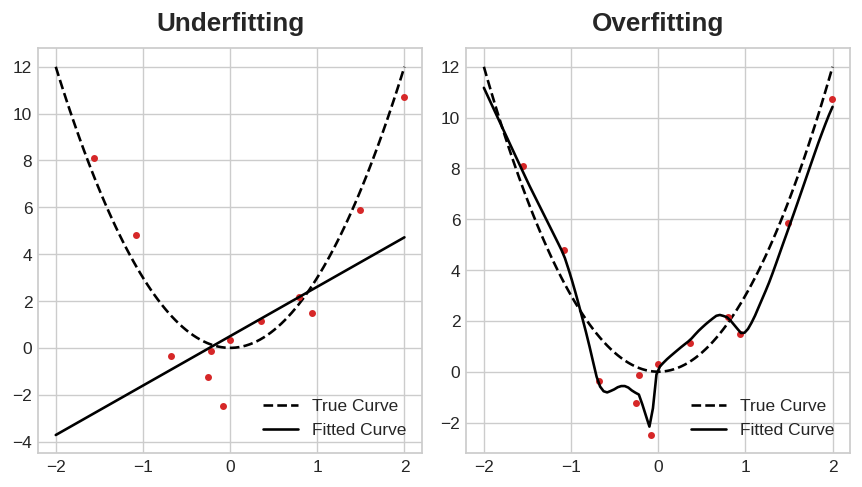
\includegraphics[width=0.7\textwidth]{underover.png}
    \caption[Underfitting and Overfitting]{Underfitting and Overfitting [\cite{holbrook}]}
    \label{fig:fitting}
  \end{center}
\end{figure}

\subsection{Missing Data}
Missing data is a problem that might also affect the quality of a dataset. It happens when no data value is stored for the variable in an observation. Missing data can significantly affect the conclusions drawn from the data.

Of course, when looking at data generation, two possible origins of missing data arise. It could be a bug of the generation software that can ultimately be corrected with due IT development. It could also be a problem in the original dataset used for the generation.

In actual datasets, missing data can occur due to a series of factors: data may be missing due to test design, failure in the observations or failure in recording observations.

\subsection{Data Imbalances}
Imbalanced data refers to datasets where the target class has an uneven distribution of observations. This is a problem in cases where small observations are relevant despite their minimal existence. For example, this can be seen in finance datasets for fraud detection, where the amount of fraud observations is very diminutive concerning the general data.

Mechanisms to prevent overfitting might increase the imbalance in the dataset as relevant data with minor occurrences could be considered noise.

\section{Data Evaluation}
For synthetic data to be considered valid, there needs to be evidence demonstrating the utility of that data. \cite{7waystodie} collected seven methods to evaluate the validity of synthetic data. Those methods are present in the following paragraphs.

The first method presented is structural similarity. Structural similarity indicates that the synthetic data should pass edit checks and have the same variable types and formats, variable names, metadata, file formats, table names and structure as real data does. The same methods used to analyse real data can be used on synthetic ones. 

General utility metrics assess general statistical parameters and model evaluation results. Using these metrics, it is also possible to assess the distinguishability between real and synthetic data. The synthetic data can be considered valid if an automated model cannot distinguish between real and synthetic data.

The utility of synthetic data can also be accessed through the replication of studies. Using this approach, we use an already-published study using the same dataset. We then replicate the results of that published study using the synthetic data. The data's validity depends on the success of the replication of results.

Letting domain experts examine the synthetic dataset and compare it to real data can also be a way to evaluate its quality. This evaluation is, however, subjective. 

Another evaluation metric is the Bias and Stability Assessment. This assessment consists of generating large quantities of synthetic datasets and calculating the general utility metrics on average. This evaluation is also valuable for evaluating the stability of the generation process.

Public available data could also be used in order to compare datasets. Synthetic datasets that reflect the same reality as publicly available real ones would be considered valid.

Comparison with Privacy-enhancing technologies is an option that can also be available. This assessment can help decision makers decide the relative strengths and weaknesses of particular PETs for providing data access.

\section{Conclusion}
In this section, we took a look at a series of methodologies and algorithms used in dataset generation. This analysis provides a series of metrics that can be helpful for the development phase.

However, bibliographic analysis of several dataset generation articles used different methods to generate datasets for other ends. We can see that each study develops its generation process per the final utilitarian purpose.

When looking at our generation, it should be noticed that application on the existing generator may not be optimal while these methodologies are helpful. The generator currently uses a configuration file that defines a series of restrictions and rules used in the synthesis. In our case, we can see that the generation process consists of an optimization problem to obey all limits while creating a dataset in the most optimal way possible. It could also be a simple generation with statistical distribution in mind. Everything depends on the configuration imputed by the user. 

Comparisons of applied improvements can be analyzed by looking at currently generated datasets generated at the end of this study using the same parameters. However, as the outcome of the generation depends on the user inputs, the system should allow for the generation of datasets of worse qualities.

We also presented ways to evaluate the quality of generated data. However, it should be noted that some of the presented evaluation methods will not be available in a purely synthetic generation.